\documentclass[a4paper,10pt]{article}

\usepackage[utf8]{inputenc}
\usepackage[slovene]{babel}
\usepackage{amsmath}
\usepackage{hyperref}
\usepackage[nottoc,numbib]{tocbibind}
\usepackage{gnuplottex}
\usepackage{graphicx}

\newcommand{\todo}[1]{(\textbf{\textsc{TODO}: #1})}

%opening
\title{Magistrsko delo}
\author{Miha \v Can\v cula}

\begin{document}

\maketitle

\section{Uvod}

\section{Opis metode}

\section{Preverjanje metode}

\subsection{Prazen prostor}

Prvi preizkus metode, ki sem ga opravil, je "sirjenje svetlobe skozi prazen prostor. 
Prazen prostor sem modeliral kot snov, kjer je dielektri"cni tenzor uniformen in izotropen. 
"Ce na eno stran celice postavimo planarni izvir ravnega valovanja, pri"cakujemo ravne valove po celotnem mediju. 

\subsection{Lom in odboj}

\subsection{Uniformen direktor}

Za naslednji preizkus sem simuliral dvolomni kristal, torej snov, kjer je dielektri"cni tenzor uniformen, ne pa tudi izotropen. 
Svetloba se je "sirila v smeri osi $z$, opti"cna os pa je oklepala kot $\theta$ z ravnino $x$-$y$ in kot $\beta$ s polarizacijo vpadne svetlobe. 
Preu"ceval sem prepustnost tak"snega sistema, "ce za celico postavimo polarizator, ki je pravokoten na polarizacijo vpadne svetlobe. 
Intenziteto prepu"s"cene svetlobe lahko izpeljemo analiti"cno\cite{kleman}, enaka je
\begin{align}
 I &= I_0 \sin^2 2\beta \sin^2 \left[ \frac{\pi d}{\lambda_0} \left( \frac{n_o n_e}{\sqrt{n_e^2 \cos^2 \theta + n_0^2 \sin^2 \theta}} - n_o \right)\right],
\end{align}
kjer sta $I_0$ in $\lambda_0$ intenziteta in valovna dol"zina vpadne svetlobe, $d$ debelina vzorca, $n_o$ in $n_e$ pa redni in izredni lomni koli"cnik. 
Ujemanje rezultatov z napovedjo je prikazano na sliki \ref{fig:test-uniform}.
\todo{vnesi parametre v graf}

\begin{figure}[h]
 \input{g_test_uniform}
 \caption{Rezultati preizkusa z uniformnim in anizotropnim dielektri"cnim tenzorjem}
 \label{fig:test-uniform}
\end{figure}

\subsection{Periodi"cna modulacija}

%bandgap => prepovedani pas, energijska re"za
Pri periodi"cni modulaciji lomnega koli"cnika opazimo pojav, da se svetloba dolo"cenih frekvenc ne more "siriti po mediju\cite{joannopoulos}. 
Temu pojavu pravimo prepovedani pas (angl. band gap). 
"Sirina in oblika tega pasu sta odvisni od obeh lomnih koli"cnikov, periode modulacije in velikosti kristala. 
Za preverjanje metode sem modeliral kristal, kjer se izmenjujejo plasti z izotropno dielektri"cnostjo $\varepsilon_1$ in $\varepsilon_2$. 
Grafa prepustnosti kristalov z razli"cnimi izbirami za dielektri"cnosti sta na sliki \ref{fig:test-periodic}. 

\begin{figure}[h]
 \input{g_test_periodic}
 \caption{Rezultati preizkusa s periodi"cno modulacijo lomnega koli"cnika}
 \label{fig:test-periodic}
\end{figure}

Na sliki res opazimo oster padec prepustnosti v dolo"cenem frekven"cnem pasu. 
Ta frekven"cni pas se dobro ujema s pri"cakovanim, ki je na sliki \ref{fig:joannopoulos-crystal}. 

\begin{figure}[h]
\centering
 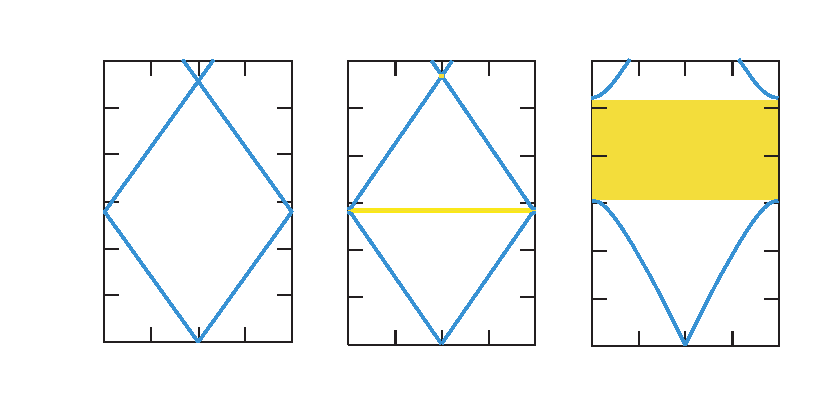
\includegraphics[width=.8\textwidth]{./Slike/bandgap}
 \caption{Pojav energijske re"za v fotonskem kristalu \todo{prepi"si iz knjige} \cite{joannopoulos}}
 \label{fig:joannopoulos-crystal}
\end{figure}

\subsection{Robni pogoji}

Za prepre"cevanje odboja na stranskih ploskvah sem uporabil absorbirajo"ce robne pogoje. 
Plast PML nam omogo"ca, da imamo material s poljubno velikimi izgubami, pa vseeno ne dobimo odboja na meji, vse dokler so elektri"cne in magnetne izgube v primernem razmerju. 
V praksi pa se zaradi diskretizacije vseeno nekaj valovanja odbije na meji med notranjostjo celice in robno plastjo. 
Najti moramo torej ravnote"zje med dvema prispevkoma: "ce so izgube majhne, bo del valovanja pri"sel skozi robno plast in se odbil na zunanjem robu. 
"Ce pa so izgube premajhne, se bo del valovanja odbil "ze na notranjem robu. 
Oba prispevka lahko zmanj"samo, "ce pove"camo debelino robne plasti, ampak s tem se pove"ca tudi "cas ra"cunanja. 
Odboj na notranji steni pa lahko omilimo, "ce se izognemo ostri meji in izgube zvezno nara"s"cajo od notranjosti proti robu. 
V literaturi\cite{taflove} priporo"cajo poten"cno nara"s"canje izgub, $\sigma \propto (d-d_0)^{p}$, kjer je $d$ oddaljenost od zunanjega roba, $d_0$ pa debelina plasti. 

Za nekaj vrednosti $p$ sem izra"cunal odbojnost robne plasti z debelino 10 enot diskretizacije. Rezultati so prikazani na sliki \ref{fig:test-absorption}. 

\begin{figure}[h]
 \input{g_test_absorption}
 \caption{Odbojnost robne plasti debeline 10 enot pri razli"cnih profilih elektri"cnih in magnetnih izgub $\sigma$. Najbolje se izka"ze material, kjer izgube nara"s"cajo kvadratno z oddaljenostjo od roba celice ($p=2$). }
 \label{fig:test-absorption}
\end{figure}

V primeru, da v plasti ni izgub, je njena odbojnost enaka 1, saj gre celotno valovanje skozi plast in se odbije na zunanji meji. 
"Ce izgume malo pove"camo, odbojnost v vseh primerih strmo pade. 
Pri profilih, kjer imamo nezveznost v izgubah ali v njihovem odvodu ($p<2$) pa odbojnost kmalu za"cne spet nara"s"cati, saj postane odboj na notranji meji "ze opazen.
Pri ve"cjih potencah pa lahko izgube "se pove"camo in s tem dose"zemo ni"zjo odbojnost plasti. 
V zgornjem primeru se za najbolj"si profil izka"ze kvadratno nara"s"canje absorpcije, zato sem za vse nadaljnje ra"cune uporabil tak"sno plast. 

\section{Rezultati}

\bibliographystyle{zumer}
\bibliography{magisterij}

\end{document}
